% Template Source: This template has been downloaded from:
% http://www.latextemplates.com/template/stylish-article
% Changed by Jelle Spijker and especcialy adapted for the
% Univeristy of applied Sciences HAN (spijker.jelle@gmail.com)
% License: CC BY-NC-SA 3.0 
%%%%%%%%%%%%%%%%%%%%%%%%%%%%%%%%%%%%%%%%%

%----------------------------------------------------------------------------------------
%	PACKAGES AND OTHER DOCUMENT CONFIGURATIONS
%----------------------------------------------------------------------------------------

\documentclass[fleqn,10pt]{SelfArx} % Document font size and equations flushed left

\usepackage{lipsum} % Required to insert dummy text. To be removed otherwise
\usepackage{animate}
\usepackage[style=numeric,citestyle=numeric,sorting=nyt,sortcites=true,autopunct=true,babel=hyphen,hyperref=true,abbreviate=false,backref=true,backend=bibtex]{biblatex}
\addbibresource{../bib.bib} % BibTeX bibliography file
\usepackage[title,titletoc,toc]{appendix}
\usepackage{listings}
\lstset{backgroundcolor=\color{color2!5}, basicstyle=\scriptsize, language=bash, moredelim=[is][\bfseries]{|}{|},classoffset=0, keywords=[1]{KEY, FOUND}, keywordstyle=[1]\color{red}\bfseries, classoffset=1, otherkeywords={!},	classoffset=0 } 
%----------------------------------------------------------------------------------------
%	REMARK ENVIRONMENT
%----------------------------------------------------------------------------------------

\newenvironment{remark}{\par\vspace{10pt}\small % Vertical white space above the remark and smaller font size
	\begin{list}{}{
			\leftmargin=35pt % Indentation on the left
			\rightmargin=25pt}\item\ignorespaces % Indentation on the right
		\makebox[-2.5pt]{
\begin{tikzpicture}[overlay]
			\node[draw=color1!60,line width=1pt,circle,fill=color1!25,font=\sffamily\bfseries,inner sep=2pt,outer sep=0pt] at (-15pt,0pt){\textcolor{color1}{R}};\end{tikzpicture}} % Orange R in a circle
		\advance\baselineskip -1pt}{\end{list}\vskip5pt} % Tighter line spacing and white space after remark
%----------------------------------------------------------------------------------------
%	COLORS
%----------------------------------------------------------------------------------------

\definecolor{color1}{RGB}{0,0,90} % Color of the article title and sections
\definecolor{color2}{RGB}{0,20,20} % Color of the boxes behind the abstract and headings
\usepackage{xcolor}

%----------------------------------------------------------------------------------------
%	TIKZ Diagrams and figures
%----------------------------------------------------------------------------------------
\usepackage{tikz}
\usetikzlibrary{arrows,shapes,positioning,shadows,trees, mindmap, matrix, calc}
\tikzset{
	basic/.style = {draw, text width=2cm, drop shadow, font=\sffamily, rectangle},root/.style = {basic, rounded corners=2pt, thin, align=center, fill=color2!30},
	level 2/.style = {basic, rounded corners=6pt, thin,align=center, fill=color1!60, text width=9em},
	level 3/.style = {basic, thin, align=left, fill=color1!8, text width=7em}
}
\tikzstyle{part} = [draw, fill=color1!20, text width=5em, text centered, minimum height= 2cm, rounded corners=12pt]
\tikzstyle{domain} = [draw, fill=color2!5, minimum height=2cm, rounded corners=12pt]
\tikzset{
	treenode/.style = {shape=rectangle, rounded corners=4pt,
		draw, anchor=center,
		text width=10em, align=center,
		color=color1!70,
		inner sep=1ex},
	decision/.style = {treenode, fill=color2!10,font=\small, diamond, inner sep=0pt, scale=0.8},
	root/.style     = {treenode, fill=color1!15},
	env/.style      = {treenode, fill=color2!5, font=\small },
	finish/.style   = {root, fill=color1!15},
	dummy/.style    = {circle,draw}
}
\newcommand{\yes}{edge node [above] {yes}}
\newcommand{\no}{edge  node [left]  {no}}

%----------------------------------------------------------------------------------------
%	HAN Variable
%----------------------------------------------------------------------------------------
\newcommand{\instutionname}{HAN University of Applied Sciences}
\newcommand{\degree}{Bachelor}
\newcommand{\studentnr}{495653}
\newcommand{\mti}{IHC MTI B.V. }
\newcommand{\vsa}{vision based sand analyzer}
\newcommand{\ihc}{Royal IHC }
\newcommand{\evd}{embedded vision design }
\newcommand{\wtb}{mechanical engineering }

%----------------------------------------------------------------------------------------
%	COLUMNS
%----------------------------------------------------------------------------------------

\setlength{\columnsep}{0.55cm} % Distance between the two columns of text
\setlength{\fboxrule}{0.75pt} % Width of the border around the abstract

%----------------------------------------------------------------------------------------
%	HYPERLINKS
%----------------------------------------------------------------------------------------

\usepackage{hyperref} % Required for hyperlinks
\hypersetup{hidelinks,colorlinks,breaklinks=true,urlcolor=color2,citecolor=color1,linkcolor=color1,bookmarksopen=false,pdftitle={Title},pdfauthor={Author}}
%----------------------------------------------------------------------------------------
%	ARTICLE INFORMATION
%----------------------------------------------------------------------------------------

\JournalInfo{\instutionname, Stage2, Period 2015-2016} % Journal information
\Archive{} % Additional notes (e.g. copyright, DOI, review/research article)

\PaperTitle{A proposal to use Github as PDM environment for a \vsa} % Article title

\Authors{Jelle Spijker\textsuperscript{1}* \studentnr} % Authors
\affiliation{\textsuperscript{1}\textit{Department of Engineering, HAN University of Applied Sciences, Arnhem, the Netherlands}} % Author affiliation
\affiliation{*\textbf{Corresponding author}: \href{mailto:spijker.jelle@gmail.com}{\color{color1}spijker.jelle@gmail.com}} % Corresponding author

\Keywords{Product Data Management --- Vision Soil Analyzer --- Github} % Keywords - if you don't want any simply remove all the text between the curly brackets
\newcommand{\keywordname}{Keywords} % Defines the keywords heading name

%----------------------------------------------------------------------------------------
%	ABSTRACT
%----------------------------------------------------------------------------------------

\Abstract{During the development of a \vsa \ or any other startup like product, it's important to manage the flow of information, such that redundancy is limited and continuity of the product(range) is guarded. This is normally done within a product data management environment (PDM). These environments normally consists of dedicated and expensive software which is supported with complex network architecture. In this article Github is explored as a free alternative for such an environment. Github is an web-based git repository service mostly used during software development. It is found that this service can be used as a full fledge free alternative PDM environment, with the use of free opensource utilities. Thus }

%----------------------------------------------------------------------------------------

\begin{document}

\flushbottom % Makes all text pages the same height

\maketitle % Print the title and abstract box

\tableofcontents % Print the contents section

\thispagestyle{empty} % Removes page numbering from the first page

%----------------------------------------------------------------------------------------
%	ARTICLE CONTENTS
%----------------------------------------------------------------------------------------

\section*{Introduction} % The \section*{} command stops section numbering
\addcontentsline{toc}{section}{Introduction} % Adds this section to the table of contents
This article proposes a setup for a PDM\footnote{Product Data Management} environment used during developed of a \vsa\footnote{Working title VSA} which analyzes sand by its optical characteristics. This new line of product(s) is currently being developed at \href{http://www.mtiholland.com/}{\color{color1}\mti} which is a R\&D based company and subsidiary of \href{http://www.ihcmerwede.com/}{\color{color1}\ihc}

The concept and initial design of this product finds it origin at the minor \evd and is developed further during the graduation phase \wtb, both taught at the \href{http://www.han.nl/international/english/}{\color{color1}\instutionname}. Design and production of this product leans on the following three disciplines: mechanical, electrical and software engineering. Due to its multidisciplinary properties it is relevant to implement a PDM environment which acts as a solid basis for all disciplines and allows for interaction and flexibility. 

The initial focus of this product where the vision algorithms written in C++, it therefore started as a software repository on \href{https://github.com/}{\color{color1}Github}, which is a web-based Git\footnote{version control system for software development designed and developed by Linus Torvalds and used for the development of the Linux Kernels} repository. Due to the changing and growing demands of this project, the focus shifted towards other engineering disciplines like electrical and mechanical. Because Git is mostly used in the development of software it is largely unknown in the mechanical engineering branch. But it is gaining traction as an PDM environment according \citeauthor{oleg_github_2013}\cite{oleg_github_2013}. 

Github is strongly rooted in software development, it therefore has a strong toolbox supporting it. This article examines the use of third party opensource software and a workflow which will ensure support for the none native disciplines: electrical and mechanical. Thus ensuring a fully fledge PDM environment. This environment will also put safeguards in-place to ensure protection of IP\footnote{Intellectual Property} but still allows multiple users/parties to work on sub-projects. It does so by defining different user roles and set restrictions to sub projects.

This article illustrate how to use Github as a PDM tool during the development of a \vsa or any startup like product. It does so by describing the normal workflow employed by Github. It will then describe the current product and give a foresight in to certain possible future developments. Afterwards it sets out the needed adjustments with respect to the normal workflow in order to support a whole startup like project such as a \vsa.

This article has the following document structure: In section \ref{sec:Vision based Sand Analyzer} the main product is described using a product breakdown structure at such a level that it

\section{Github}\label{sec:Github}
\href{https://github.com/}{\color{color1}Github} is a web-based Git repository hosting service with SCM\footnote{Source Code Management} and distributed revision control capabilities. It also provides access control and multiple collaboration features, such as bug tracking, feature request, task management and wikis. Github has a strong influence in the open-source community. This is because standard "free" services don't allow for private repositories. They're accessible by all and thus allow everyone to view, copy and use them. A lot of company, governments and institutions such as NASA, CERN, Google and Netflix do so under the credo; Dare to share. 
For those whom want to protect their intellect property they offer paid accounts which allow for private repositories. It is also possible to host your own service using \href{https://about.gitlab.com/}{\color{color1}GitLab} 

Recent developments show a move from strictly software support to other disciplines, to cite \citeauthor{peter_bell_introducing_2015} \cite{peter_bell_introducing_2015} While GitHub is still primarily used to collaborate on the development of software, it’s also a great way for a team to collaborate on a wide range of projects. From the authoring of books and the distribution of models for 3D printing to the crafting of legislation, whenever you have a team of people collaborating on a collection of documents, you should consider using Github to manage the process.

Github is based on the Git workflow, which was developed by Linus Torvald to help with the development of the Linux kernels. Git is a strict command-line tool which emphasizes on speed and data integrity, it allows for a distributed, non-linear workflow. This workflow is explained in the next section.

\subsection{The normal Github workflow}\label{sec:nomal github workflow}
As mentioned in the previous sections, Github is Git-based and works with repository which can roughly be described as a directory structure with revision control. This workflow is depicted in figure \ref{fig:gitworkflow} and can be described as follows: A new repository is created on the remote server, which is then pulled to a local host. A user can make changes in this directory by adding, deleting or modifying files and directories. Each alteration such as the addition of a few lines of code, which represent a new function are added to the staging area. These alterations are then committed to the current branch, which will be discussed further on. These commits are then pushed to the remote server, where they're stored with meta-data such as comment, blame (who applied the change), and a date. Each commit only stores the change in the file and allows a user to review against previous commits (versions). 

If another developer has committed new work, the developer first has to pull these changes to his local host before he is allowed to push his own changes. Git will automatically detect any conflicts and show them to the developer. He will then be allowed to solve these conflicts if needed.

\begin{figure}[t]
	\includegraphics[width=\textwidth/2]{../images/githubworkflow1.png}
	\caption{Git workflow. Source: \citeauthor{_git_2015} \cite{_git_2015}}\label{fig:gitworkflow}
\end{figure}

As mentioned before the commits are first stored in a branch. These branches allow for distributive workflow. They do so be running parallel with the master branch. If a new feature is being developed, it is common practice to create a new branch, implement the new features, which probably consist of multiple commits and pushes to the remote server. Which allow other developers to work on the same feature as needed. All the while changes are still allowed on the master or any other branch. Once the feature is ready to be added to the master or an other branch, a pull request is made to the community.

This will compare the current branch against the other branch and allow for other developers to discus and review the code. If they find it satisfactory and they don't foresee any major problems the pull request is granted and the branch is merged. This process is shown in figure \ref{fig:branchworkflow}.

\begin{figure}[ht]\centering
	\includegraphics[width=\textwidth/2]{../images/stepup.png}
	\caption{Distributive workflow with branches. Source: \citeauthor{backlog_branching_2015}\cite{backlog_branching_2015} }\label{fig:branchworkflow}
\end{figure}

The figure \ref{fig:branchworkflow} also shows the use of tags. It is possible for a developer to tag a certain commit, in essence freezing the state of the project. This is mostly done when versions are released to the public or classification agencies. These tags allow the  state of the project to be recalled at that time.

\subsection{Issues}
Further active collaboration is supported and encouraged using Issues. These a generic items which could be idea's, task, bug reports or questions for instance, which can be submitted by a developer. An issue is created by describing it, illustrating it with images, links or examples. Assigning a label to it such as ToDo, bug, feature enhancement. Other developers can comment on these issues so as to give it direction. Such an issue and discussion is shown in figure \ref{fig:issue}. These issues can be assigned to individual developers and be assigned to milestones. Which allows them to focus on further goals.

\subsection{Project wiki}
Each project has its own wiki\footnote{A wiki is a website which allow sharing of knowledge by collaborative modifications} It's expected from the developers to maintain an active wiki. All knowledge regarding the project can be gathered here, shared and improved

\section{Vision based Sand Analyzer}\label{sec:Vision based Sand Analyzer}
The \vsa is a product that analyzes sand sample using a digital camera sensor. It does so by taking a snapshot of a magnified soil sample and applying multiple software algorithms on an obtained digital image. A detailed and full description of the first two prototypes are described in the product documentations of the previous build prototypes \cite{jelle_spijker_vision_2015} and \cite{spijker_product_2014}, where the last iteration serves as the basis for the product breakdown structure depicted in the next subsection.

\subsection{Product breakdown structure VSA}
The product breakdown structure, depicted in figure \ref{fig:PBSVSA} differentiates between three structures: hardware, software and the casing. This demarcation is made to better serve the different disciplines. This breakdown is purely done on individual parts, where each part serves a function. The intricate web of interfaces and connections are set out in section \ref{sec:Interfaces}.

Due to the scope of this document these functions are not specified. The software functionality is covered in detail in the \href{http://peer23peer.github.io/VisionSoilAnalyzer/Doxygen/html/index.html}{\color{color1}Doxygen documentation}. It is important to note that the software is developed with the object orientated language C++ and is divided in different namespaces. Which are depicted in figure \ref{fig:PBSVSA}. Each of these namespaces is a bundle of object each serving its own function and by inheritance it's possible to create complex objects. Integration of the software development environment in Github is seamless.

Whilst function which are fulfilled by the casing and hardware are describes in the product documentations \cite{jelle_spijker_vision_2015}. The individual parts serve as actuators, sensors and interfaces with the outside world.  

\begin{figure*}[h]\centering
	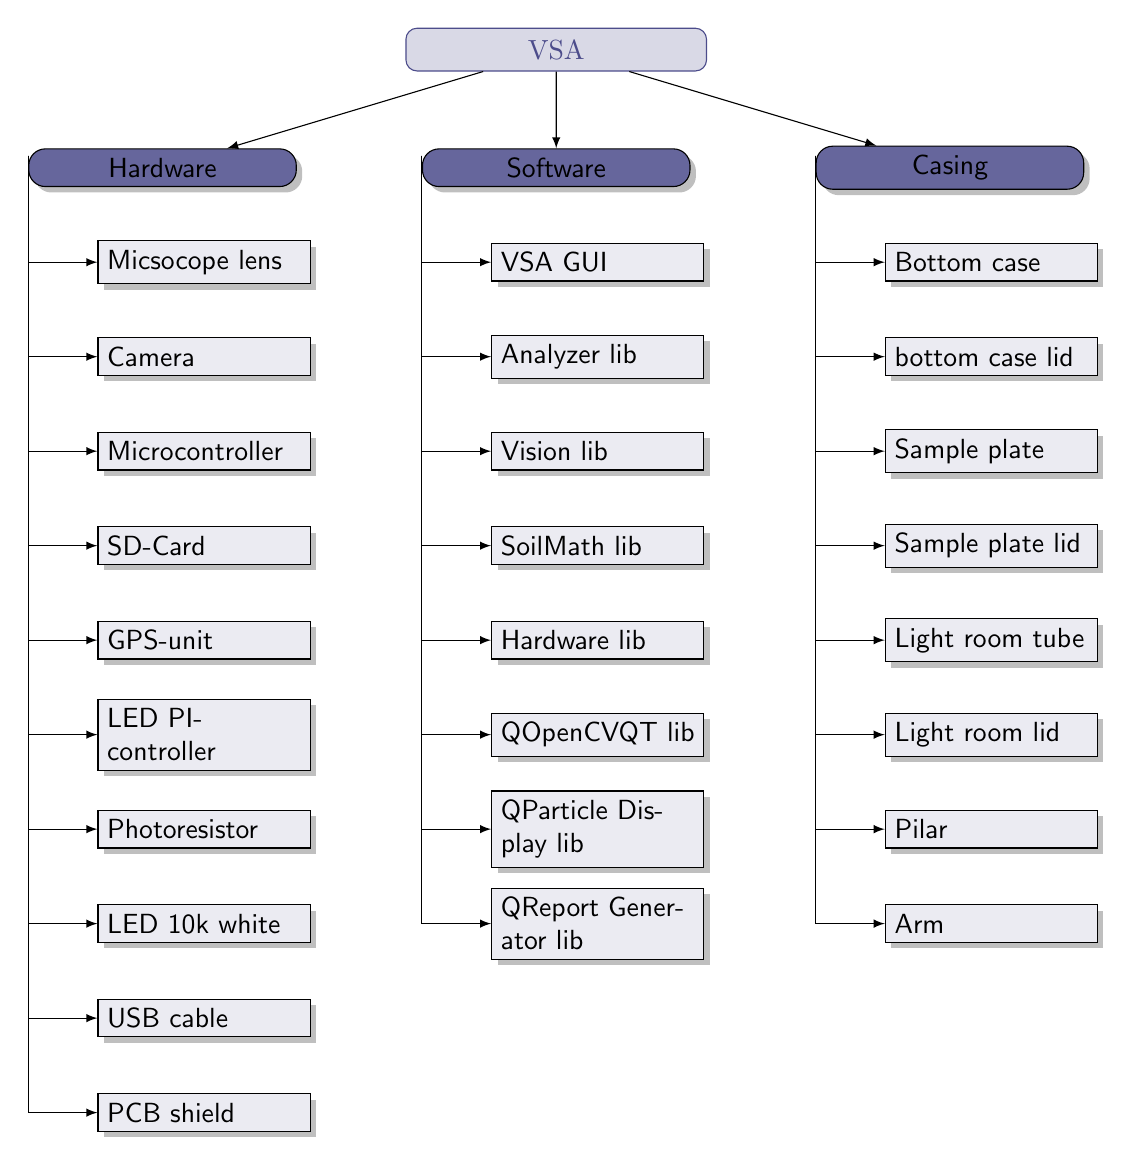
\begin{tikzpicture}[level 1/.style={sibling distance=50mm}, edge from parent/.style={->,draw},>=latex]
	\node[root] {VSA}
	child {node[level 2] (c1) {Hardware}}
	child {node[level 2] (c2) {Software}}
	child {node[level 2] (c3) {Casing}};
	
	\begin{scope}[every node/.style={level 3}, node distance=12mm]
		\node[below of = c1, xshift=15pt] (c11) {Micsocope lens};
		\node[below of = c11] (c12) {Camera};
		\node[below of = c12] (c13) {Microcontroller};
		\node[below of = c13] (c14) {SD-Card};
		\node[below of = c14] (c15) {GPS-unit};
		\node[below of = c15] (c16) {LED PI-controller};
		\node[below of = c16] (c17) {Photoresistor};
		\node[below of = c17] (c18) {LED 10k white};
		\node[below of = c18] (c19) {USB cable};
		\node[below of = c19] (c110) {PCB shield};
		
		\node[below of = c2, xshift=15pt] (c21) {VSA GUI};
		\node[below of = c21] (c22) {Analyzer lib};
		\node[below of = c22] (c23) {Vision lib};
		\node[below of = c23] (c24) {SoilMath lib};
		\node[below of = c24] (c25) {Hardware lib};
		\node[below of = c25] (c26) {QOpenCVQT lib};
		\node[below of = c26] (c27) {QParticle Display lib};
		\node[below of = c27] (c28) {QReport Generator lib};
		
		\node[below of = c3, xshift=15pt] (c31) {Bottom case};
		\node[below of = c31] (c32) {bottom case lid};
		\node[below of = c32] (c33) {Sample plate};
		\node[below of = c33] (c34) {Sample plate lid};
		\node[below of = c34] (c35) {Light room tube};
		\node[below of = c35] (c36) {Light room lid};
		\node[below of = c36] (c37) {Pilar};
		\node[below of = c37] (c38) {Arm};		
	\end{scope}
	
	\foreach \value in {1,...,10}
	\draw[->] (c1.175) |- (c1\value.west);
	
	\foreach \value in {1,...,8}
	\draw[->] (c2.175) |- (c2\value.west);

	\foreach \value in {1,...,8}
	\draw[->] (c3.175) |- (c3\value.west);

	\end{tikzpicture}
	\caption{Product breakdown structure of VSA v1.0}\label{fig:PBSVSA}
\end{figure*}

\subsection{The toolboxes}\label{sec:Toolboxes}
Each discipline uses it's own type of tools, it is therefore relevant to asses all used tools and make sure the are compatible with each other. Each of the tools below are stand-alone versions which run on a operating system, they store their data in files, which in turn can be seen as the output. At the basis of all three development environments lies the hardware. The specifications given below, describe the current development computer. It is guaranteed that the project can be recreated with a similar computer.
\begin{itemize}[noitemsep]
	\item Intel(R) Core(TM) i5-4210U CPU @ 1.70GHz
	\item 8gb memory
	\item Nvidia 820M
	\item SSD 128 gb
	\item HDD 500 gb
	\item Dual boot with Kubuntu 15.10 / Windows 10
\end{itemize}

\paragraph{Software engineering}
The VSA currently runs on a dedicated embedded Linux environment and is programmed in C++. The IDE\footnote{Integrated Development Environment} consist of a Linux Debian environment running \href{http://www.qt.io/}{\color{color1}Qt Creator}, testing is done with \href{http://valgrind.org/}{\color{color1}Valgrind} and code compiling is done with the \href{https://gcc.gnu.org/}{\color{color1}GNU GCC compiler} or \href{http://clang.llvm.org/}{\color{color1}LLVM Clang}.
The basic list of used libraries is given below.
\begin{itemize}[noitemsep]
	\item Standard C++ Library
	\item OpenCV 3.0 beta
	\item CUDA 7.0 SDK
	\item ZLib
	\item Boost 1.58
	\item Video4Linux
	\item GStreamer
\end{itemize}

All these packages are chosen such that the can easily be ported to other operating systems, such as Windows, Android or iOS. Although current prototypes are dedicated embedded devices, the ultimate goal is to create a cheap and portable device. In order to achieve that goal, it is important to make use of existing and readily available architecture such as phones and laptop. Software development has to be done with this foresight; Currently all these tools allow for this strategy.

The output of the software engineering toolbox will be mostly source code and binary files. The source code files are plain text format, which can be read and edited from most devices. While the binary files will consist of images and other additional resources needed by the program. This actual program needs to be compiled for each individual target system. This is done with each release and the files are bundled with the version tag.

Future release may save their data in databases, it is possible that these database run on the local host, but they could also run on remote host. Databases need special care to put under Git revision control. The best practice is to dump the database and schema and put the output -- which is a plain text file -- under git control.
	
\paragraph{Electrical engineering}
The actuators and sensors, such as the GPS-unit, LEDs and photoresistor are all driven from an embedded Linux device, The \href{http://beagleboard.org/BLACK}{\color{color1}Beaglbone Black}. This device has the capability to run an OS and can interact with the outside world by pinmuxing\footnote{Changing the state and function of pins on the CPU, such that it allows for different in- output protocols}. The PCB\footnote{Printed Circuit Board} and circuits are designed with the \href{http://sine.ni.com/nips/cds/view/p/lang/nl/nid/204744}{\color{color1}Circuit Design Suite} from National Instruments.

This suite consist of the programs \href{http://www.ni.com/multisim/}{\color{color1}Multisim} for circuit design \& simulation and \href{http://www.ni.com/ultiboard/}{\color{color1}Ultiboard} for PCB design. Both programs only run in a Windows environment. Multisim works with a binary file with the extension \textit{*.ms14}, but it also has an option to output SPICE\footnote{Simulation Program with Integrated Circuit Emphasis}. Which are plain text files, and can be used with a multitude of different simulation programs. Ultiboard works with a binary file that has the extension \textit{*.ewprj}. It can export in the Gerber format, which is a plain text file and the de facto industry standard used with PCB.

\paragraph{Mechanical engineering}
Each part has a mechanical representation. These parts are modeled in \href{http://www.plm.automation.siemens.com/nl_nl/products/nx/}{\color{color1}Siemens NX 10}, which offers a rich interface for mechanical engineers. They allow for parametric modeling and complex FEM and CFD simulations. Siemens NX output all its file in binary formats. These files aren't backward compatible.

Github recently adopted a new viewer for 3D-models. It can now read and compare previous versions of \textit{*.stl} files, as shown in figure \ref{fig:view}. These file are easily exported with NX and are used for CAM\footnote{Computer Aided Manufacturing} such as CNC\footnote{Computer Numerical Control}, 3D-printing or any other rapid-prototyping technique.

\begin{figure}[ht]\centering 
	\animategraphics[loop,autoplay,width=\textwidth/2]{12}{../images/githubframe-}{0}{34}
	\caption{Revision control of 3D models, source: \citeauthor{skalnik_3d_2013}\cite{skalnik_3d_2013}}
	\label{fig:view}
\end{figure}

Simulations and calculations are done with \href{http://nl.mathworks.com/products/matlab/}{\color{color1}Matlab 2015a}, which has a Git integration. Most Matlab files are plain text files, but special care should be taken with the Simulink models. According to the Matlab website it is necessary to prevent Git from corrupting Simulink models, this is done by editing the \textit{.gitattributes} file and adding the following lines: 
\begin{lstlisting}{bash}
	*.slx -crlf -diff -merge
	*.mdl -crlf -diff -merge
	*.mat -crlf -diff -merge
	*.mlx -crlf -diff -merge
\end{lstlisting}

\paragraph{Documentation}
All documentation is written with \LaTeX, which is a word processor and a mark-up language. Documents are written in plain text files with macro command in between, which -- when compiled with the \LaTeX compiler generate typeset documents. These output documents are stored as \textit{*.pdf} files. This document is an example of such an output file.

\subsection{Interfaces}\label{sec:Interfaces}
Each part has an interfaces, which describe how it interacts with other parts. This project defines interfaces in four domains; These are: mechanical, electrical, software and corporate. The last one represent the interface with (after-)sales and supply chain.  Not all domains are represented for each part, but a part should have at least one interface, otherwise it is redundant.

Each part in the project has a fully defined interface. Due to the limited scope of this article only the interface used with the \href{http://www.lumileds.com/products/high-power-leds/luxeon-rebel}{\color{color1}LED Luxeon Rebel} is used as an example. This is shown in figure \ref{fig:interfaces}.

\begin{figure*}[!ht]\centering
	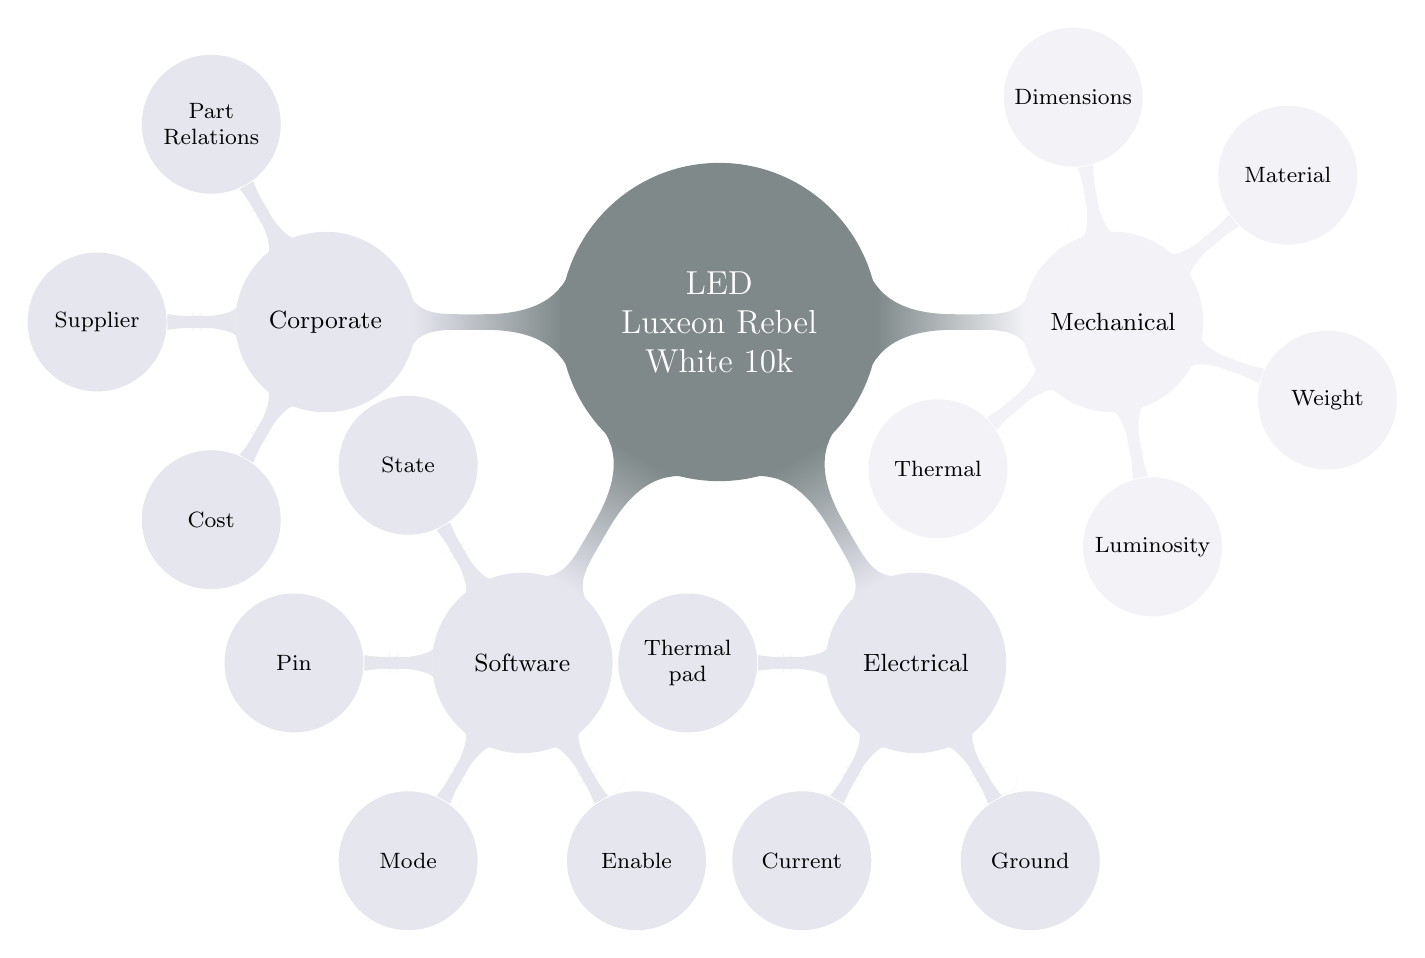
\begin{tikzpicture}
		\path[mindmap,concept color=color2!50, text=white]
		node[concept] {LED \\ Luxeon Rebel \\ White 10k}
		[clockwise from=0]
		child[concept color=color2!5!color1!5, text=black] {
			node[concept] { Mechanical }
			[clockwise from=100]
			child { node[concept] { Dimensions } }
			child { node[concept] { Material } }
			child { node[concept] { Weight } }
			child { node[concept] { Luminosity } }
			child { node[concept] { Thermal } }
			}
		child[concept color=color2!5!color1!10, text=black] {
			node[concept] { Electrical }
			[clockwise from=-60]
			child { node[concept] { Ground } }
			child { node[concept] { Current } }
			child { node[concept] { Thermal pad } }
			}
		child[concept color=color2!5!color1!10, text=black] {
			node[concept] { Software }
			[clockwise from=-60]
			child { node[concept] { Enable } }
			child { node[concept] { Mode } }
			child { node[concept] { Pin } }
			child { node[concept] { State } }
			}
		child[concept color=color2!5!color1!10, text=black] {
			node[concept] { Corporate }
			[clockwise from=-120]
			child { node[concept] { Cost } }
			child { node[concept] { Supplier } }
			child { node[concept] { Part Relations } }
			};
	\end{tikzpicture}
	\caption{Interface of a Luxeon Rebel 10k LED}\label{fig:interfaces}
\end{figure*}

\section{What is a PDM environment}
In order to truly understand a PDM environment, one has to start with the main definition, which is according to \citeauthor{la_product_2009} \cite{la_product_2009} a strategy which puts the right product and process related information in the right hands at the right time in a product life cycle. It also allows for the creation of processes which guard those data en allows other to use it. All the while generating en secure environment, at which all relevant information, and previous iterations is stored without redundancy.

Github is without a doubt a great tool when used as revision control it save all relevant information and stores it in a secure environment without redundancy. It has potential to be used as a full fledge PDM environment. But in order to maximize Github for this setup it is relevant to look at the mechanics of such an environment a little closer, so that it becomes clear what should be added or changed.

\paragraph{Data vault}
Each data item should be stored in one single location, where only authorized developers can access that data at a time when its needed. In order to support this system, roles should be defined. Each developer needs to be assigned one or more roles, which allows him access the for that role relevant data. The role should also specify if he has read or modification rights.

\paragraph{Metadata}
One of the main features of a PDM environment is a possibility to quickly look-up metadata\footnote{Data about data}, which comes in two flavors: structural and descriptive. The structural metadata tells something about the container e.g. a file, whilst descriptive meta-data gives a user information with regards to the data content. Searching for this data should be intuitive and simple; Using elementary queries.

\paragraph{Classification}
Classification of the files is important because not every file uses the same metadata fields. Classification can be done with the use of (sub)groups, narrowing the possibilities and making sure only the relevant items turn up in a search. It is advised to also create a classification system per functionality.

\paragraph{Check-in / -out}
Developers should not disturb each others workflow. They check-out their work, modify it, and check it in again; Accompanied with a small description of the changes.

\paragraph{Bill of materials}
A complete list of all materials should be easily obtained for each product, preferably from different role perspectives.

\paragraph{Configuration management}
Configuration management is registering and administrating all kinds of information, during the development process. It is central that certain states of the development process can be obtained when needed; So called snapshots.

\paragraph{Design review}
During the design process it is paramount that certain choices, comments and agreements are saved and can be accessed at any time. This helps when there is a need to review certain parts of the design.

\paragraph{Data visualization}
Not every user has all development programs accessible, but it could be possible that he needs information 
 
\section{Implement Github as PDM environment}
When the traditional services of Github are set against the requirements for a PDM environment, certain deviations become apparent. This missing functionality can be implemented using free third-party opensource solutions such as \href{http://tmsu.org/}{\color{color1}TMSU}. A utility which allows files to be tagged with meta data.

\subsection{Meta tagging with TMSU}
The tagged files can be accessed through a virtual mounted file system. Which allows the use of queries and lets them browse through the obtained results as if it where directories. This allows maximum compatibility with other software. TMSU also has the option to assign a value to meta tag. It's therefore possible to create a tag "Length" with a value for that a specific part. This allows for configuration management, such as the bash\footnote{linux console output} print out below illustrates. TMSU is at is core a Linux program and runs on Debian based distributions. It can be compiled for Windows but without the option of a virtual mounted file system.

The use of TMSU tags and queries is illustrated below. In this example all metric $ 8[mm] $ parts are shown. With the first command all parts are shown, but the second query only shows the part that tests true for all values. The workings of TMSU are further illustrated in a \href{https://youtu.be/bvwW0buxSD4}{\color{color1}screencast}.

\begin{figure}[!hb]
	\begin{lstlisting}{bash}
	$ tmsu files "m=8"
	./3Dmodel/parts_pdm/bolt_m8_50_316L
	./3Dmodel/parts_pdm/bolt_m8_50_s235jr
	./3Dmodel/parts_pdm/bolt_m8_60_316L
	./3Dmodel/parts_pdm/bolt_m8_60_s235jr
	./3Dmodel/parts_pdm/bolt_m8_70_316L
	./3Dmodel/parts_pdm/bolt_m8_70_s235jr
	./3Dmodel/parts_pdm/washer_m8_316L
	./3Dmodel/parts_pdm/washer_m8_s235jr
	./3Dmodel/parts_pdm/nut_m8_316L
	./3Dmodel/parts_pdm/nut_m8_316L
	
	$ tmsu files "m=8 and material=s235jr and length=50"
	./3Dmodel/parts_pdm/bolt_m8_50_s235jr
	\end{lstlisting}
	\caption{TMSU query on the command line}
\end{figure}


Best practice is to define all four domain interfaces (mechanical, electrical, software and corporate) as valued meta tags. This way all relevant interfaces can be found with a simple query. Each defined value in a domain interface, illustrates a meta tag in its own right. This assures compatibility with other parts. Since the structure for each file is defined. This will ensures easy linking and matching of individual parts.

By extending Github with TMSU it is possible to use classification, create a bill of materials, use configuration management and define inter-parts relations. Thus it becomes a full fledge PDM. But it's a fragile connection. Much depends on the naming of meta tags and the users work flow. The following workflow has proven to work.

\subsection{Binary workflow new feature}
In order to minimize the disturbance of the main product, new features are added with branches. As explained before in section \ref{sec:nomal github workflow} a branch is just branch; It is a offshoot of the master branch at a certain point such that modifications and changes are implemented. This branch can be merged at a later point with the master branch. 

Although Github is steadily implementing certain features for binary files, such as \textit{*.stl} support it's still best to work with a different workflow, when working with binary files. This is because the difference can't be ascertained by Github. These need to manually determined by the developers. This process is shown in appendix \ref{fig:workflow new feauture}.

This is when the corporate interface domain comes in handy. Each file that is connected  to another needs to be linked in the relations interface. This meta tag needs to be updated by the developer. That way a simple query can show the impact certain changes have on the whole design and which developers need to be notified in the suggested change. By opening up an issue, and assigning the work to the responsible developers. The dialog between them ensures an compatible new feature. 

\subsection{Project planning}
The use of issues and milestones enable a fluent project planning which is up-to-date with the latest workload. In order to distribute this load it is possible to use the third party service \href{https://waffle.io}{\color{color1}Waffle}, which integrates completely with Github. It shows the status of all issue, and present four column, namely: Backlog, Ready, In Progress and Done. All open issue start in the Backlog, when preparations are made to start working on them to can be moved to the Ready column. As soon as work is commenced the move to the In Progress column, when they're finished the move towards the Done column. The throughput of the project can be monitored closely allowing to actively steer on optimal team performance. 
\begin{figure}[!hpt]
	\centering
	\includegraphics[width=\textwidth*\real{0.5}]{../images/waffle.png}
	\caption{Waffle project planning}\label{fig:waffle}
\end{figure}
\section{Results and Discussion}
\lipsum[5-8]

%----------------------------------------------------------------------------------------
%	REFERENCE LIST
%----------------------------------------------------------------------------------------
%\clearpage
\phantomsection
\printbibliography

%----------------------------------------------------------------------------------------
\phantomsection
\appendix
\newpage
\onecolumn
%\renewcommand\thesection{\Alph{section}}
\section*{Appendices}
\addcontentsline{toc}{section}{Appendices}
\renewcommand{\thesubsection}{\Alph{subsection}}
\subsection{Workflow add binary feature}
\centering
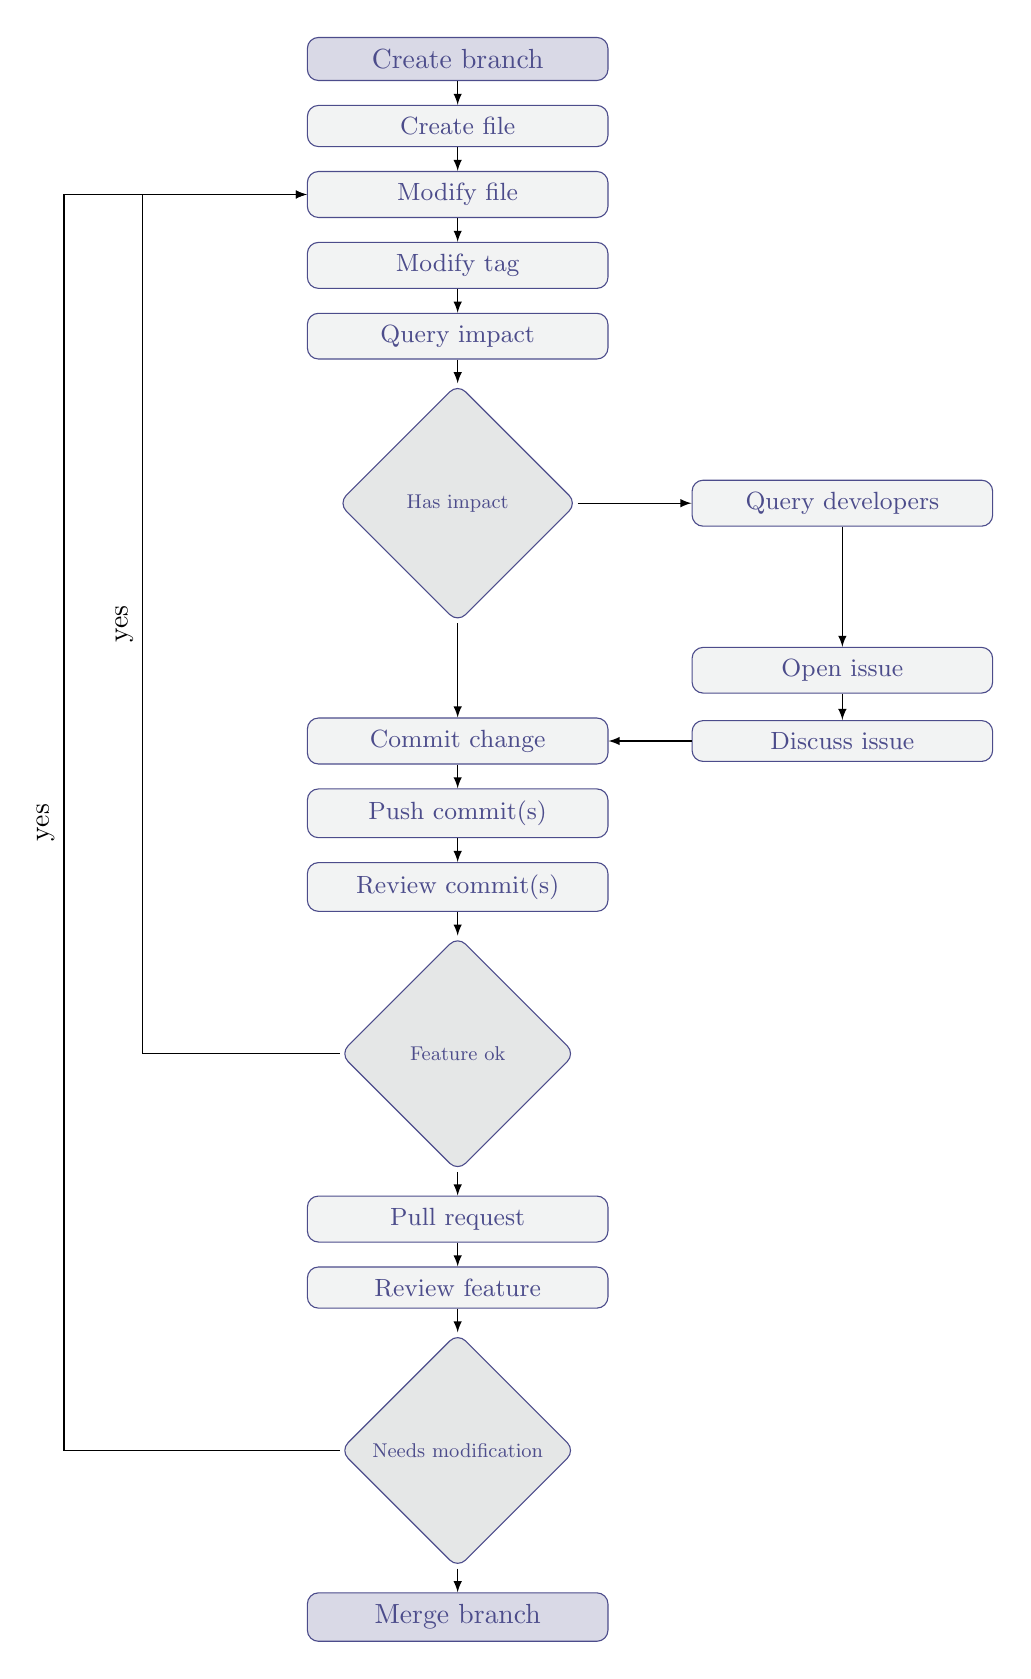
\begin{tikzpicture}[-latex]
\matrix(chart)
[
matrix of nodes,
column sep = 3em,
row sep = 2ex
]
{
	|[root]| Create branch 	& \\
	|[env]| Create file 		& \\
	|[env]| Modify file 		& \\
	|[env]| Modify tag		& \\ 
	|[env]| Query impact 		& \\
	|[decision]| Has impact 	& |[env]| Query developers \\
	& |[env]| Open issue \\
	|[env]| Commit change	    & |[env]| Discuss issue \\
	|[env]| Push commit(s)	& \\
	|[env]| Review commit(s)	& \\
	|[decision]| Feature ok & \\
	|[env]| Pull request & \\
	|[env]| Review feature & \\
	|[decision]| Needs modification & \\
	|[finish]| Merge branch & \\	
	};
	\draw
	(chart-1-1) edge (chart-2-1)
	(chart-2-1) edge (chart-3-1)
	(chart-3-1) edge (chart-4-1)
	(chart-4-1) edge (chart-5-1)
	(chart-5-1) edge (chart-6-1)
	(chart-6-1) edge (chart-8-1)
	(chart-6-1) edge (chart-6-2)
	(chart-6-2) edge (chart-7-2)
	(chart-7-2) edge (chart-8-2)
	(chart-8-2) edge (chart-8-1)
	(chart-8-1) edge (chart-9-1)
	(chart-9-1) edge (chart-10-1)
	(chart-10-1) edge (chart-11-1)
	(chart-11-1) edge (chart-12-1)
	(chart-12-1) edge (chart-13-1)
	(chart-13-1) edge (chart-14-1)
	(chart-14-1) edge (chart-15-1);
	\draw
	(chart-11-1) -- +(-4,0) |- (chart-3-1)
	node[near start, sloped, above] {yes};
	\draw
	(chart-14-1) -- +(-5,0) |- (chart-3-1)
	node[near start, sloped, above] {yes};
	
	\end{tikzpicture}
	\label{fig:workflow new feauture}
\end{document}